\section{Introduction}
Modeling is a powerful tool in synthetic biology. It can provide us with an important engineering approach to characterize our pathways quantitatively and predict their performance, thus help us test and modify our design.

Through the dynamic model, we hope to gain insights of the characteristics of our whole circuit's dynamics. Several tools including ODEs and interpolation are employed.


\section{Method}

\begin{figure}[h]
\centering
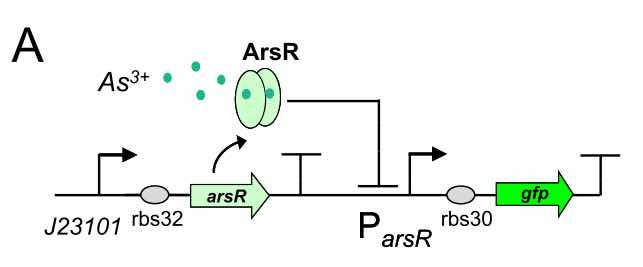
\includegraphics[width=12cm,height=5cm]{1}
\caption{Schematic diagram of plasmid1}
\end{figure}

At the beginning, on the plasmid\#1, the promoter $P_{arsR}$ isn't bound with ArsR, thus it is active. $ArsR$ and $smURFP$ are transcribed and translated under the control of the promoters $P_{arsR_u}$ and $P_{arsR_d}$, with subscript $u$ and $d$ representing upstream and downstream separately. The subscript $l$ of smURFP in the equation means leaky expression without the expression of $As^{3+}$. As ArsR is expressed gradually, it will bind with the promoter $P_{arsR}$ and make it inactive. 

\begin{equation}
P_{J23104} \stackrel{k_1}{\longrightarrow} P_{J23104}+ArsR
\end{equation}
\begin{equation}
P_{arsR_d} \stackrel{k_2}{\longrightarrow} P_{arsR_d} +smURFP_l
\end{equation}

\begin{equation}
ArsR+P_{arsR} \xrightleftharpoons[k_{-3}]{k_3}ArsR*P_{arsR} 
\end{equation} 

On the plasmid\#2, the fusion protein of dCas9 and RNAP(RNA polymerase) are produced after transcription and translation, and $sgRNA$ is produced after transcription.

\begin{equation}
P_{tet} \stackrel{k_{4}}{\longrightarrow} P_{tet} +dCas9*RNAP
\end{equation}
\begin{equation}
P_{tet} \stackrel{k_{5}}{\longrightarrow} P_{tet} +sgRNA
\end{equation}

\begin{figure}[h]
	\centering
	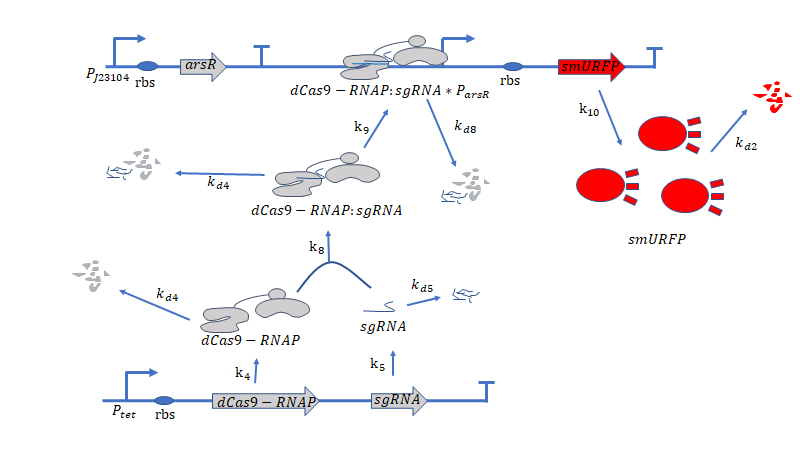
\includegraphics[width=12cm,height=5cm]{2}
	\caption{Schematic diagram of dCas9/RNAP}
\end{figure}

dCas9(*RNAP) can bind with its target DNA sequence without cutting, which is at the upstream of the promoter $P_{arsR_d}$. Simultaneously, dCas9 can lead RNAP to bind with the promoter $P_{arsR_d}$ and enhance the transcription of smURFP. However, because the promoter $P_{arsR_d}$ has already bound with ArsR, as a result, RNAP can't bind with the promoter $P_{arsR_d}$ . \\ 

However, at the presence of $As^{3+}$, it can bind with ArsR, then dissociate ArsR and $P_{arsR_d}$, which makes the combination of RNAP and $P_{arsR_d}$ possible. \\

(Declaration: $[dCas9/RNAP] = [dCas9] = [RNAP]$;\\ $[P_{arsR_d}]=[P_{arsR_u}] = \frac{1}{2}[P_{arsR}]$ )

\begin{equation}
ArsR +As^{3+}\xrightleftharpoons[k_{-6}]{k_6}As^{3+}*ArsR
\end{equation}
\begin{equation}
ArsR*P_{arsR} +As^{3+}\xrightleftharpoons[k_{-7}]{k_7}P_{arsR}+ As^{3+}*ArsR
\end{equation}
\begin{equation}
dCas9*RNAP+sgRNA\xrightleftharpoons[k_{-8}]{k_8} dCas9*RNAP:sgRNA
\end{equation}
\begin{equation}
dCas9*RNAP:sgRNA+P_{arsR_d}\xrightleftharpoons[k_{-9}]{k_9} dCas9*RNAP:sgRNA*P_{arsR_d}
\end{equation}
\begin{equation}
dCas9*RNAP:sgRNA*P_{arsR_d}\stackrel{k_{10}}{\longrightarrow} dCas9*RNAP:sgRNA*P_{arsR_d}+smURFP
\end{equation}
\\
We then take degradation into account:\\
\begin{equation}
ArsR\stackrel{k_{d1}}{\longrightarrow}Ø
\end{equation}

\begin{equation}
smURFP\stackrel{k_{d2}}{\longrightarrow}Ø
\end{equation}


\begin{equation}
ArsR*P_{arsR}\stackrel{k_{d3}}{\longrightarrow}P_{arsR}
\end{equation}

\begin{equation}
As^{3+}*ArsR\stackrel{k_{d4}}{\longrightarrow}As^{3+}
\end{equation}

\begin{equation}
dCas9*RNAP\stackrel{k_{d5}}{\longrightarrow}Ø
\end{equation}

\begin{equation}
sgRNA\stackrel{k_{d6}}{\longrightarrow}Ø
\end{equation}

%\begin{equation}
%dCas9-RNAP:sgRNA\stackrel{k_{d7}}{\longrightarrow}dCas9-RNAP
%\end{equation}

\begin{equation}
dCas9*RNAP:sgRNA\stackrel{k_{d7}}{\longrightarrow}Ø
\end{equation}

%\begin{equation}
%dCas9-RNAP:sgRNA*P_{arsR}\stackrel{k_{d8}}{\longrightarrow}dCas9-RNAP+P_{arsR}
%\end{equation}

\begin{equation}
dCas9*RNAP:sgRNA*P_{arsR}\stackrel{k_{d8}}{\longrightarrow}P_{arsR}
\end{equation}
\\\\
\begin{table}[htbp]
	\centering
	\caption{\label {tab:test} Parameters}
	\begin{tabular}{cccccccccccccccccc}
		\toprule
		Rate constants & Value& units \\
		\midrule
		k1 & 1.999e-5 &1/s \\
		k2 & 3.312e-6 &1/s \\
		k3 & 3.3e7    & 1/M    \\
		k4 &1.995e-5 &1/s\\
		k5 & 3.312e-6 &1/s \\
		k6 &1.66e7   &1/M  \\
		k7  &1.26e4 &1/s  \\
		k8&1.6e-2& 1/s\\
		k9 &1.66e-5&1/s\\ 
		k10&4e-5&1/s\\
		kd1 & 3.07e-3&1/s\\
		kd2&1e-5&1/s\\
		kd3&1e-3&1/s\\
		kd4&1.53e-3&1/s\\
		kd5 & 2e-2&1/s\\
		kd6&7.62e-3&1/s\\
		kd7& 1e-2&1/s\\
		kd8&1e-1&1/s\\		
		\bottomrule
	\end{tabular}
\end{table}



\subsection{simulation }
\begin{figure}[h]
	\centering
	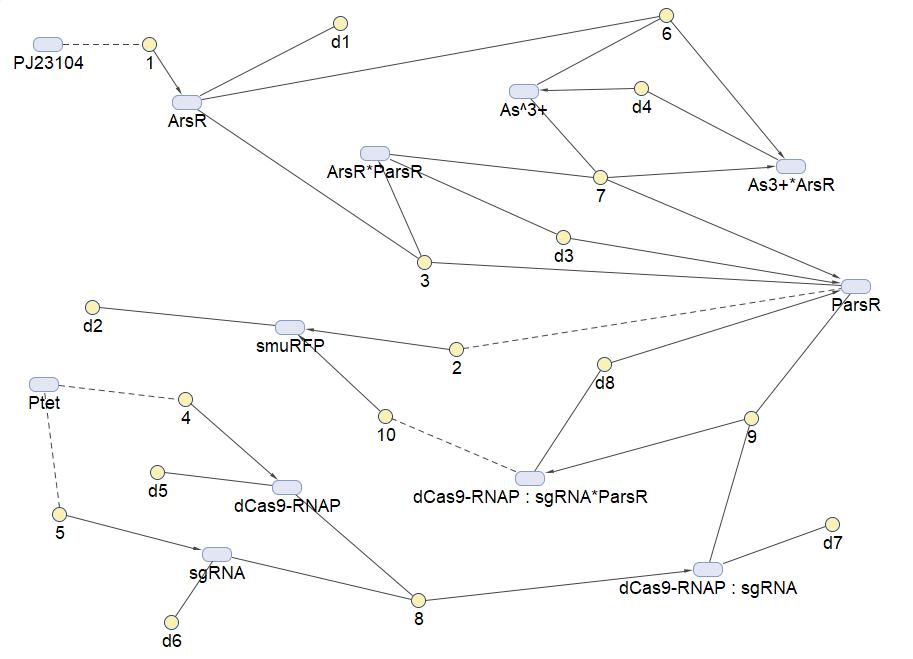
\includegraphics[width=10cm,height=7cm]{screenshot003}	
	\caption{reaction map generated from the reaction set above using SimBiology Toolbox}
\end{figure}
SimBiology toolbox provides functions for modeling, simulating, and analyzing biochemical pathways on basis of the powerful computing engine of Matlab.

\begin{figure}[h]
	\centering
	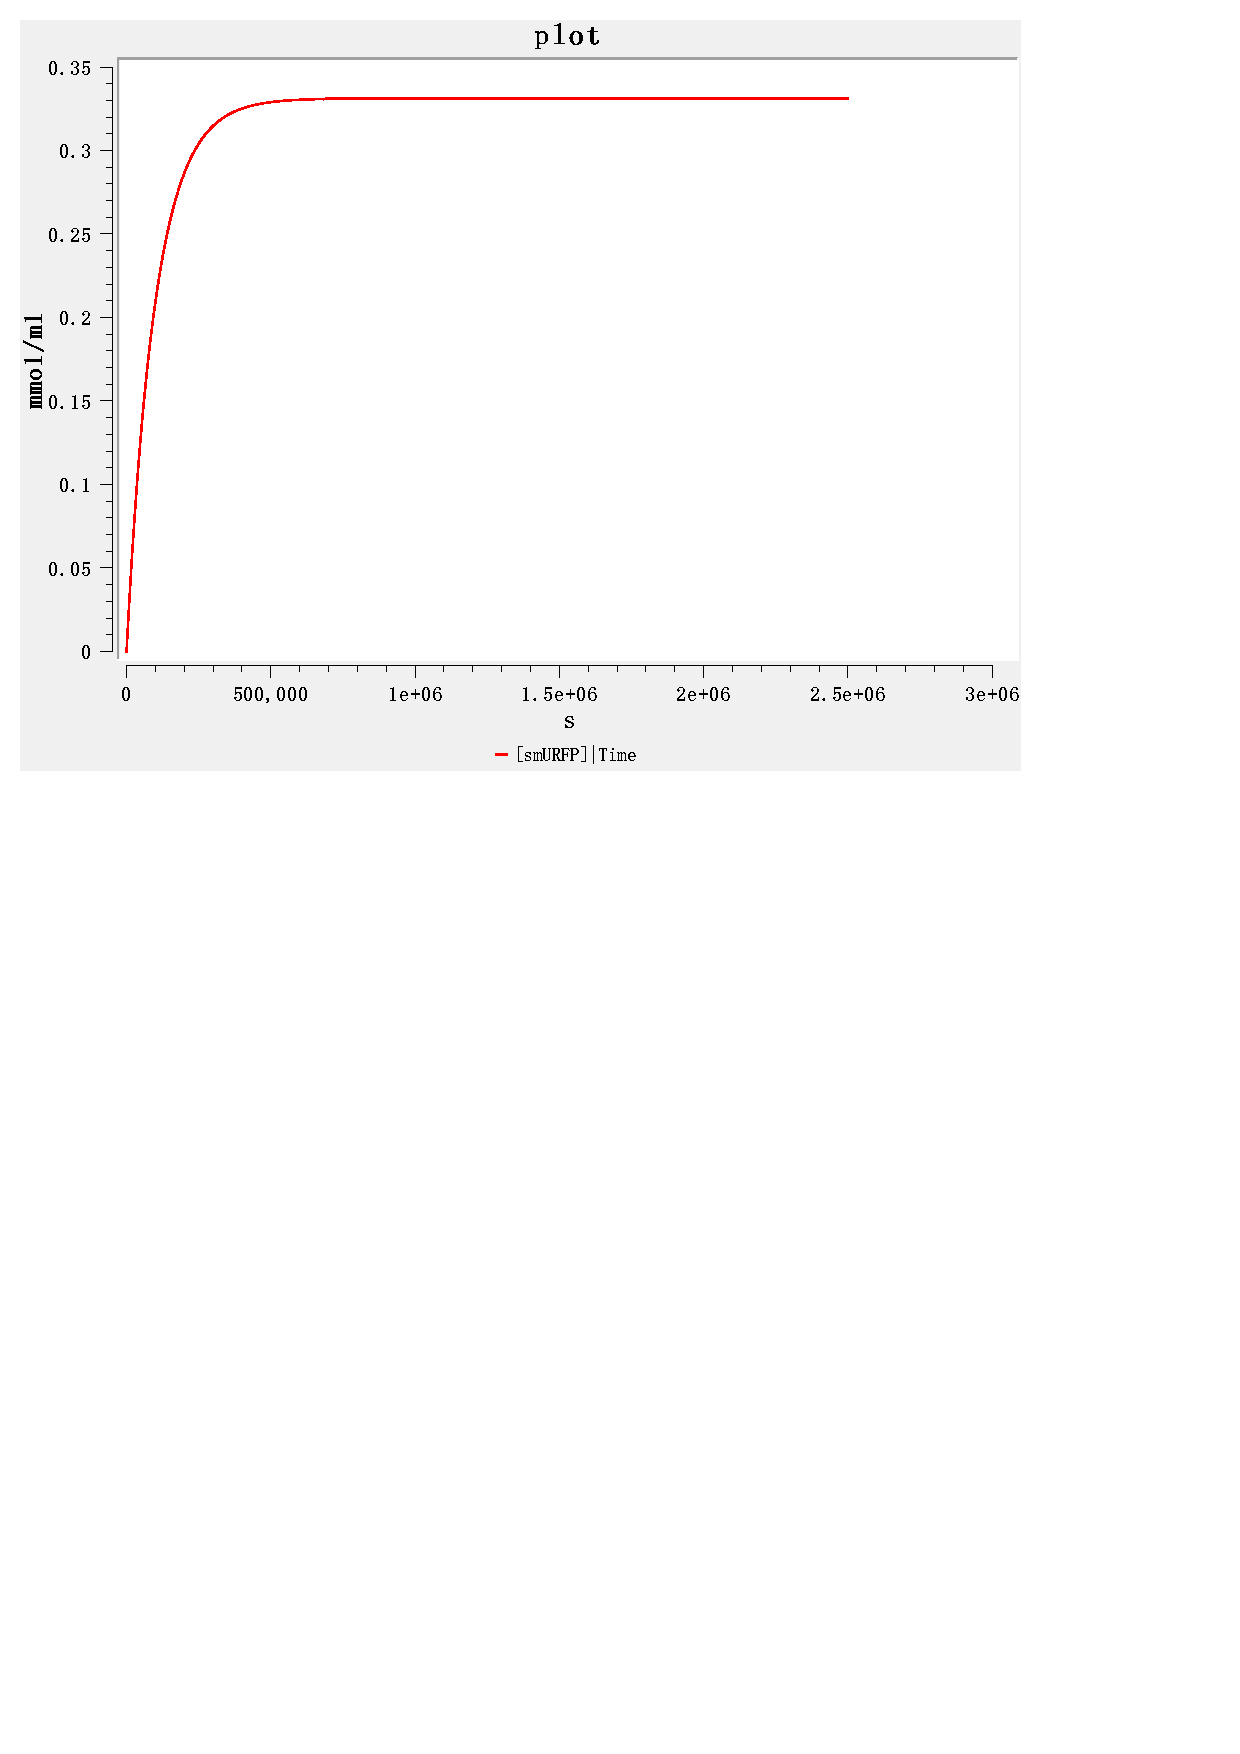
\includegraphics[width=10cm,height=10cm]{smuRFP}
	\caption{Schematic diagram of smURFP fluorescence by COPASI}
\end{figure}



COPASI is freeware developed withcollaboration of VBI and EMLR. It provides
almost the same functions as SimBiology, though not quite powerful. But compared with SimBiology, it provides a friendly user interface for model analysis, such as parameter estimation,and parameter scan.

Through the figure, we can see that the smURFP fluorescence gradually increased and then reached a steady state after a period of time  in the presence of arsenic ions.

\section{References} 
1.Berset, Y. et al. Mechanistic Modeling of Genetic Circuits for ArsR Arsenic Regulation. ACS Synthetic Biology 6, 862–874 (2017).\\

2.Bikard, D.et al. Programmable repression and activation of bacterial gene expression using an engineered CRISPR-Cas system. Nucleic Acids Research 41, 7429–7437 (2013).\\

3.Cai, Y. et al. Modeling the arsenic biosensor system. BMC Systems Biology 1, P83 (2007).\\

4.Pola-López, L. A. et al. Novel arsenic biosensor “POLA” obtained by a genetically modified E. coli bioreporter cell. Sensors and Actuators B: Chemical 254, 1061–1068 (2018).

\end{document}






